\documentclass{article}
\usepackage{amsmath}
\usepackage{amssymb}
\usepackage{amsmath}
\usepackage{enumitem}
\usepackage{hyperref}
\usepackage{graphicx}
\usepackage{subcaption}
\usepackage[margin=1in]{geometry}

\renewcommand{\v}{\mathbf}
\title{MATH 408 Project Proposal}
\author{Ben Young}
\begin{document}
\pagenumbering{gobble}
	\maketitle
    For my project I plan to undertake a general exploration of lattice-based cryptography: the math behind it and its applications, especially regarding its potential resistance to quantum-based attacks.
    I also hope to implement an algorithm to solve a common lattice problem, such as the shortest vector problem.
    \\

    A \textit{lattice} is essentially the set of all linear combinations of a given set vectors with linear coefficients. 
    More formally, if $\v{b}_1,\cdots,\v{b}_n \in \mathbb{R}^n$ are $n$ linearly independent basis vectors 
    we can define a lattice $\mathcal{L}$ as
\begin{equation*}
    \mathcal{L}(\v{b}_1,\cdots,\v{b}_n) = \left\{\sum_{i=1}^n{x_i\v{b}_i : x_i \in \mathbb{Z}}\right\}
    \footnote{D. Micciancio and O. Regev. ``Lattice-based Cryptography''. 22 July 2008. cims.nyu.edu/$\sim$~regev/papers/pqc.pdf}
\end{equation*}
\begin{figure}[h!]
    \caption{An example of a 2-dimensional lattice with basis vectors [1]}
    \centering
    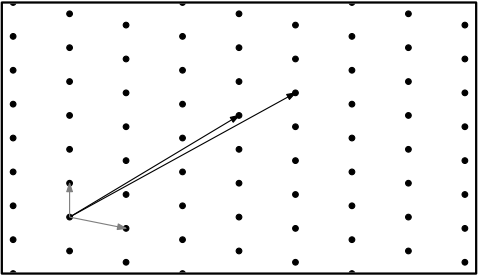
\includegraphics[scale=0.3]{lattice.png}
\end{figure} \\
One common lattice-related problem is to find the length of the shortest vector that can be created from the basis. This is the \textit{shortest vector problem}.
As with most lattice problems, algorithms aim to find an approximation
of the solution within a factor of the actual length of the shortest vector. Several algorithms exist, although none have both polynomial runtime and approximation factor. The \textit{LLL algorithm} runs in 
polynomial time but achieves only a $O(2^n)$ approximation factor.
Every known algorithm that finds an exact solution or a polynomial approximation has running time $O(2^n)$. 
Furthermore, it is conjectured that there exists no polynomial time algorithm (quantum or classical) that can approximate the shortest vector problem
or other lattice problems to within a polynomial factor.
Other problems include the \textit{closest vector problem}, which asks for the closest lattice point to a target non-lattice vector,
and the \textit{shortest independent vectors problem}, which asks for the set of linearly independent lattice vectors with the smallest
maximum length.\footnotemark[\value{footnote}]\\

The hardness of lattice problems and their resistance to quantum attacks have led to several proposed cryptosystems, although most are
too inefficient to be used in practice. 
One such cryptosystem is the GGH cryptosystem. Public and private keys are two
different bases for the same lattice. The public key is a `good'
basis which allows for effeciently solving some cases
of the closest vector problem. The public key is a `bad' basis which
is much less efficient for solving the same problem. 
A different approach is the \textit{learning with errors} (LWE) cryptosystem.
The system is based on the lattice problem with the same name. 
Given a basis for a random lattice and a vector $\v{v} \in \mathbb{Z}^m_q$ ($m$-length vectors mod $q$), decide
whether $\v{v}$ is chosen randomly and uniformly from $\mathbb{Z}^m_q$ or if it was chosen by randomly perturbing the coordinates of
a point in the lattice.\footnotemark[\value{footnote}]
\end{document}
